%------------------ vorlage.tex ------------------------------------------------
%
% LaTeX-Vorlage zur Erstellung von Projektdokumentationen
% im Fachbereich Informatik der Hochschule Trier
%
% Basis: Vorlage 'svmono' des Springer Verlags
% Bearbeiter: Hermann Schloß, Christian Bettinger
%
%-------------------------------------------------------------------------------


%------------------ Präambel ---------------------------------------------------
\documentclass[envcountsame, envcountchap, deutsch]{i-studis}

\usepackage[utf8]{inputenc}

\usepackage[a4paper]{geometry}
\usepackage[english, ngerman]{babel}

\usepackage[pdftex]{graphicx}
\usepackage{epstopdf}

\usepackage{listings}

\usepackage[german, ruled, vlined]{algorithm2e}
\usepackage{amssymb, amsfonts, amstext, amsmath}
\usepackage{array}
\usepackage[skip=10pt]{caption}
\usepackage[usenames, dvipsnames]{color}
\usepackage[pdftex, plainpages=false]{hyperref}
\usepackage{textcomp}

\usepackage{bibgerm}
\bibliographystyle{geralpha}

\usepackage{makeidx}
\usepackage{multicol}
\makeindex

\pagestyle{myheadings}
\setlength{\textheight}{1.1\textheight}

\lstset{
	basicstyle=\scriptsize\ttfamily,
	commentstyle=\scriptsize\ttfamily\color{Gray},
	identifierstyle=\scriptsize\ttfamily,
	keywordstyle=\scriptsize\ttfamily,
	stringstyle=\scriptsize\ttfamily,
	tabsize=4,
	numbers=left,
	numberstyle=\tiny,
	numberblanklines=false,
	frame=single,
	framesep=3mm,
	framexleftmargin=7mm,
	xleftmargin=10mm,
	linewidth=144mm,
	captionpos=b,
}


%------------------ Manuelle Silbentrennung ------------------------------------
\hyphenation{Ele-men-tar-ob-jek-te ab-ge-tas-tet Aus-wer-tung House-holder-Matrix Least-Squares-Al-go-ri-th-men}


%------------------ Titelseite -------------------------------------------------
\begin{document}

\title{Entwicklung einer Hotelbuchungssoftware}
\subtitle{Development of hotel booking software}

\author{Alexander Falkenberg, Hasan Alhelal}

\supervisor{Titel Vorname Nachname}

\address{Ort}
\submitdate{DD.MM.YYYY}

%------------------ Projektart -------------------------------------------------
%\project{Bachelor-Projektarbeit}
\project{Teamprojekt}
%\project{Master-Projektstudium}
%\project{Master-Abschlussarbeit}
%\project{Seminar}
%\project{Hausarbeit}

\mytitlepage

%------------------ Vorwort, Kurzfassung, Verzeichnisse ------------------------
\frontmatter					% Vorwort (optional)
\kurzfassung

Das Thema der Ausarbeitung ist das Erstellen einer Webseite für das fiktive Grandline Hotel mit Standort in der Vulkaneifel. Die Webanwendung soll dem Unternehmen ermöglichen, Zimmerbuchungen online anzubieten. Dadurch soll der Prozess des Buchens oder Abänderns einer bereits getätigten Buchung erleichtert und dem Kunden alle nötigen Informationen dargeboten werden. Ziel ist es, den Umsatz des Unternehmens durch mehr Buchungen zu steigern.
\\
\\ 
Zuerst müssen die Grundlagen für den client- und den serverseitigen Teil der Anwendung gelegt werden. Dazu zählen die Grundlagen von HTML, Less, JavaScript/Node.js usw. Anschließend werden einige Konzepte dargestellt und die Implementierung der Anwendung beschrieben. Um die Buchung umzusetzen, wird eine API mithilfe von Express in Node.js implementiert. Es wird außerdem eine beispielhafte Benutzung der Anwendung dargestellt und weitere Szenarien aufgezeigt, in denen man ein solches Buchungssystem gebrauchen kann. Schlussendlich wird die Arbeit zusammengefasst und ein Ausblick für weitere Verbesserungen gegeben.

\kurzfassungEN

The topic of the paper is the creation of a website for the fictional Grandline Hotel located in the Vulkaneifel region. The web application should enable the company to offer room bookings online. This should make the process of booking or changing an already made reservation easier and provide the customer with all necessary information. The goal is to increase the company's revenue through more bookings.
\\
\\
First, the fundamentals for both the client-side and server-side parts of the application need to be established. This includes the basics of HTML, Less, JavaScript/Node.js, and so on. Afterwards, some concepts will be presented and the implementation of the application will be described. To implement the booking, an API will be implemented using Express in Node.js. Additionally, an exemplary usage of the application will be demonstrated, and other scenarios in which such a booking system could be useful will be presented. Finally, the work will be summarized, and an outlook for further improvements will be provided.
							% Kurzfassung/Abstract
\tableofcontents										% Inhaltsverzeichnis
\listoffigures											% Abbildungsverzeichnis (optional)


%------------------ Kapitel ----------------------------------------------------
\mainmatter
\chapter{Einleitung}
\section{Motivation}
Diese Arbeit handelt von der Umsetzung eines Buchungssystems für ein Hotel. Ein solches System ist besonders wichtig um den allgemeinen Aufwand beim Verwalten von verfügbaren Zimmern deutlich zu verringern und der Fehleranfälligkeit beim Vergeben von eben diesen vorzubeugen. Außerdem kann diese Software in leicht abgeänderter Form auch problemlos für andere Anwendungen benutzt werden.


\section{Ziele der Arbeit}
Ziel dieser Arbeit ist es ein simples Buchungssystem zu schaffen dass sich ohne großen Arbeitsaufwand verwenden lässt. Es soll den Nutzern des Systems möglich sein ohne die Erstellung eines Nutzerprofils Buchungen tätigen und diese verwalten zu können. Die Informationen über jede Buchung werden den Nutzern anschließend per Email zugesandt.
\input{chapters/VerwandteArbeiten}
\chapter{Grundlagen}

\section{HTML, CSS, JS}
\subsection{HTML}
\subsection{Less}
\subsection{JavaScript}

\section{Node.js}
Die serverseitige Grundlage des Systems bildet die Laufzeitumgebung Node.js. Mit dieser ist es möglich JavaScript Programme abseits eines Browsers ausführen zu können. Mithilfe von \glqq npm\grqq, dem Paketmanager von Node.js, werden außerdem externe Pakete für bestimmte Funktionalitäten verwendet um die Implementierung zu vereinfachen.

\subsection{Express}
Das Express-Framework ermöglicht eine unkomplizierte Erstellung einer Webanwendung. So wird beispielsweise die Verarbeitung von HTTP-Anfragen wird mithilfe von spezifischen Methoden deutlich vereinfacht und macht das Erstellen einer API besonders effizient. Innerhalb der Buchungssoftware sorgt Express für die Bereitstellung eines Servers, der alle clientseitigen Dateien zur Verfügung stellt und auf HTTP-Anfragen zur Erzeugung oder zum Abrufen von Buchungen, reagiert.

\subsection{Nodemailer}
Nodemailer ist ein \glqq npm\grqq-Paket, das dafür verwendet wird E-Mails mit Node.js zu versenden. Durch Angabe der Adresse von der die E-Mail verschickt werden soll und verschiedenen Optionen wie z.B. dem Betreff wird das Senden vereinfacht. Um eine E-Mail zu versenden muss im ersten Schritt ein \glqq Transporter\grqq zusammen mit dem verwendeten Mail Dienst und den Anmeldeinformationen der zu sendenen E-Mail Adresse, erzeugt werden. Anschließend werden die Mail-Optionen initialisiert und über die Methode \glqq sendMail\grqq des Transportes, die E-Mail versandt.

\subsection{Formidable}

\section{MongoDB}
Unter den dokumentenorientierten NoSQL-Datenbanken ist MongoDB die meist verwendete. Die wichtigsten Bestandteile einer MongoDB Datenbank sind Dokumente und Collections. Dokumente sind Datenstrukturen die sich aus einem oder mehreren Paaren, bestehend aus Feldern und dazugehörigen Werten, zusammenfügen. In ihrem Aufbau sind diese Dokumente identisch mit JSON Objekten. Collections hingegen sind Sammlungen von verschiedenen Dokumenten und sind vergleichbar mit Tabellen aus relationalen Datenbanken.
\\
\\
Damit eine Node.js-Anwendung mit einer MongoDB kommunizieren kann wird beispielsweise das \glqq npm\grqq-Paket \glqq mongodb\grqq benötigt. Hier können dann auf den einzelnen Collections, Methoden angwendet werden. Die wichtigsten Methoden für das zu erstellende System sind \glqq find\grqq , \glqq insertOne\grqq , \glqq deleteOne\grqq und \glqq deleteMany\grqq. Mithilfe von find werden alle Dokumente einer Collection geliefert, auf die ein in der Methode spezifiziertes Kriterium zutrifft. InsertOne ermöglicht es ein neues Dokument in eine Collection hinzuzufügen und deleteOne bzw. deleteMany ermöglicht das Löschen von Dokumenten aus einer Collection.

\chapter{Konzept}
Das folgenden Bild beschreibt den groben Aufbau der Anwendung und die Technologien die auf den verschiedenen Ebenen verwendet wird.
\begin{figure}
	\includegraphics[width=0.8\textwidth]{images/Architektur.png}
	\centering
	\caption{Grobe Architektur des Systems}
\end{figure}

Die Sitemap dient dazu die Navigation durch die  Anwendung und den Zusammenhang der einzelnen Unterseiten darzustellen.
\begin{figure}
	\includegraphics[width=0.8\textwidth]{images/Sitemap.png}
	\centering
	\caption{Sitemap}
\end{figure}
\newpage
Diese Abbildung stellt den Aufbau der Datenbank dar, wobei jedes Rechteck eine Collection abbildet mit Dokumenten die jeweils die Ovale als Attribute besitzt.

\begin{figure}
	\includegraphics[width=\textwidth]{images/Datenbank.png}
	\caption{Datenbankentwurf}
\end{figure}

Dieser Algorithmus spielt in der finalen Implementierung eine wichtige Rolle, da in vielen Fällen die verfügbaren Zimmer bestimmt werden müssen.
\begin{algorithm}
	\caption{Algorithmus um alle verfügbaren Räume zu erhalten}\label{alg:one}
	\KwData{rooms = alle Räume,
		reservations = alle Buchungen,
		arrival = Anreisedatum,
		departure = Abreisedatum
	}
	\KwResult{available = verfügbare Räume}
	$notAvailable \gets [\thinspace]$; \newline
	\For{room of rooms}{
		\For{reservation of reservations}{
			\If{$(room.id == reservation.room) \thickspace \&\& \thickspace !(departure < reservation.arrival \thickspace || \thickspace arrival > reservation.departure)$}{
				notAvailable.push(room);\newline
				break;
			}
		}
	}

    \Return{$available = rooms.filter(item \thickspace => \thickspace !notAvailable.includes(item))$}
\end{algorithm}
\chapter{Realisierung}


\chapter{Implementierung}
\section{Dreidimensionale Zimmer}
\chapter{Beispiele}
Im Folgenden wird eine beispielhafte Interaktion eines Nutzers mit dem System anhand von Bildschirmabzügen erläutert. In diesem Szenario will der fiktive Nutzer eine Buchung für Zimmer in dem Grandline-Hotel tätigen. Im ersten Schritt besucht der Nutzer die Startseite und klickt auf den \glqq buchen\grqq-Knopf (siehe Abb.\ref{step1}).
\begin{figure}
	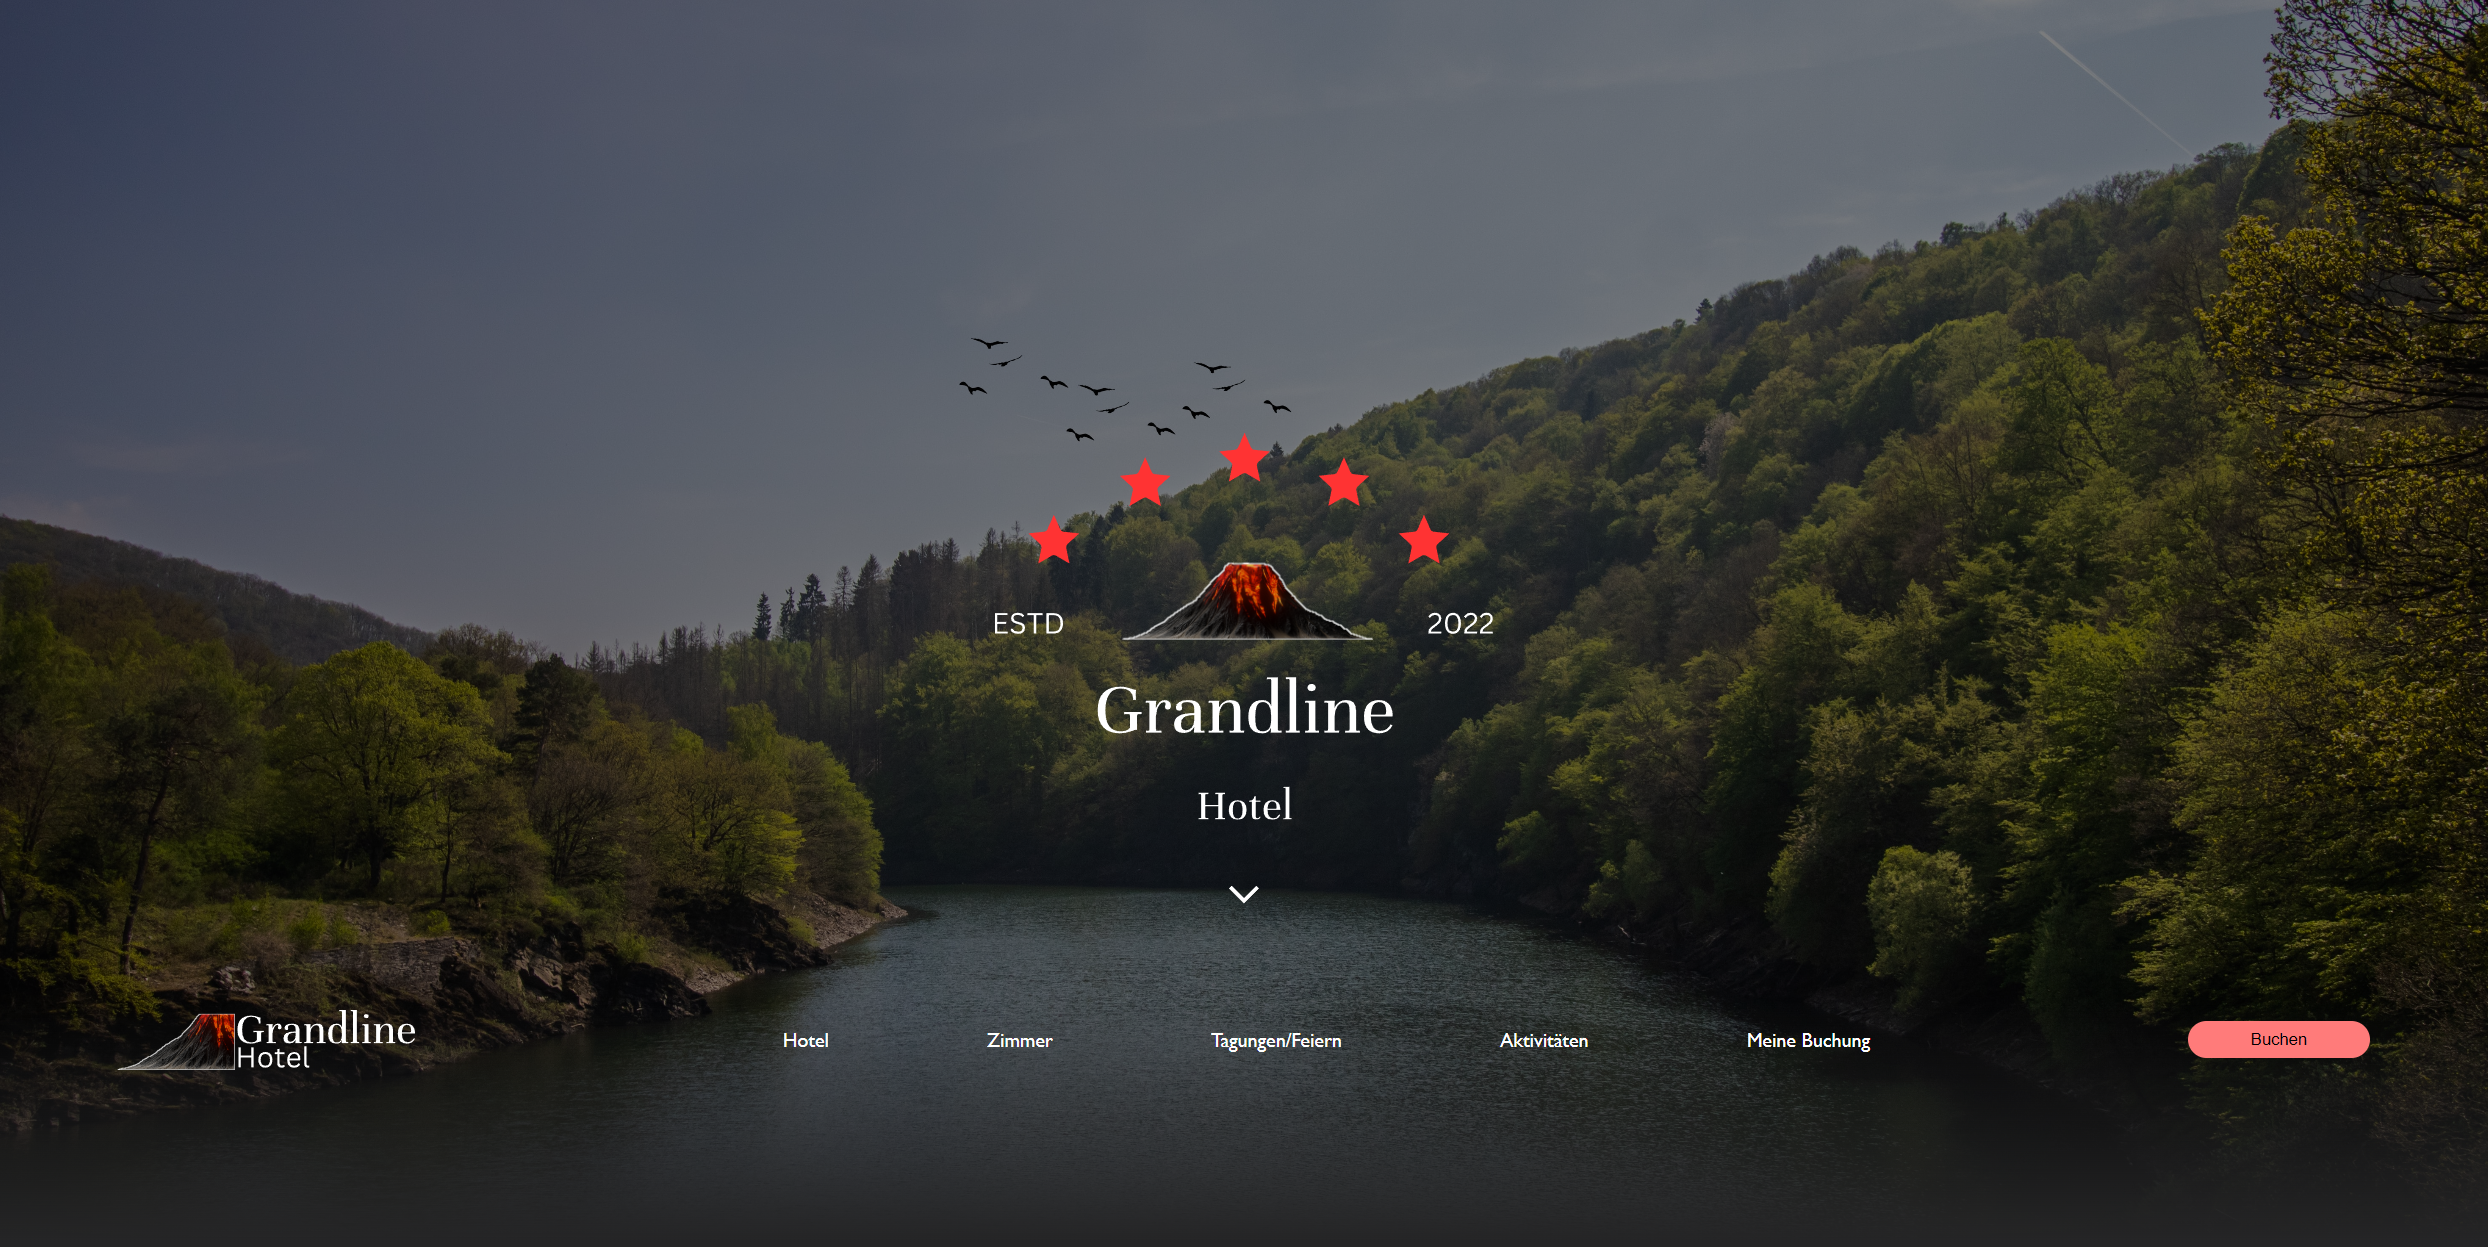
\includegraphics[width=\textwidth]{images/Beispiel/Schritt1.png}
	\caption{Schritt 1}
	\label{step1}
\end{figure}
\newline
Als Folge des Klicks auf den \glqq buchen\grqq-Knopf kommt ein Formular (siehe Abb.\ref{step2}) hervor in welchem der Nutzer die Reisedaten und Anzahl der Zimmer für die gewünschte Buchung angeben kann.
\begin{figure}
	\includegraphics[width=\textwidth]{images/Beispiel/Schritt2.png}
	\caption{Schritt 2}
	\label{step2}
\end{figure}
\newpage In dem 3.Schritt tätigt der Nutzer seine Angaben in das Formular und setzt durch einen Klick auf den \glqq weiter\grqq-Knopf mit der Buchung fort (siehe Abb.\ref{step3}).
\begin{figure}
	\includegraphics[width=\textwidth]{images/Beispiel/Schritt3.png}
	\caption{Schritt 3}
	\label{step3}
\end{figure}
\newline
Der Nutzer wird nun in den Buchungsdialog weitergeleitet in dem er eine Auswahl der verfügbaren Zimmer dargeboten bekommt (siehe Abb.\ref{step4}).
\begin{figure}
	\includegraphics[width=\textwidth]{images/Beispiel/Schritt4.png}
	\caption{Schritt 4}
	\label{step4}
\end{figure}
\newpage
Der Nutzer wählt im 5. Schritt aus den verfügbaren Zimmern die Gewünschten aus und betätigt die \glqq Weiter\grqq-Taste (siehe Abb.\ref{step5}). Die Menge die der Nutzer auswählen muss entspricht der angegebenen Anzahl der Zimmer aus Schritt 3.
\begin{figure}
	\includegraphics[width=\textwidth]{images/Beispiel/Schritt5.png}
	\caption{Schritt 5}
	\label{step5}
\end{figure}
\newpage
In das nun erschienene Formular trägt der Nutzer seine persönlichen Daten ein und fährt über den \glqq Weiter\grqq-Knopf mit dem Buchungsdialog fort (siehe Abb.\ref{step6}).
\begin{figure}
	\includegraphics[width=\textwidth]{images/Beispiel/Schritt6.png}
	\caption{Schritt 6}
	\label{step6}
\end{figure}
\newline
Im siebten Schritt wird dem Nutzer eine Übersicht über die zu tätigende Buchung dargeboten und bietet dem Nutzer vor dem Abschluss die Möglichkeit noch Extrawünsche und Informationen über ein Textfeld an das Hotel weiterzugeben (siehe Abb.\ref{step7}). Klickt der Nutzer anschließend auf \glqq Abschließen\grqq, wird der Buchungsprozess abgeschlossen.
\begin{figure}
	\includegraphics[width=\textwidth]{images/Beispiel/Schritt7.png}
	\caption{Schritt 7}
	\label{step7}
\end{figure}
\newpage
Nach Abschluss der Buchung wird der Nutzer darüber informiert, dass eine E-Mail mit den wichtigsten Informationen an den Nutzer versendet wurde (siehe Abb.\ref{step8}).
\begin{figure}
	\includegraphics[width=\textwidth]{images/Beispiel/Schritt8.png}
	\caption{Schritt 8}
	\label{step8}
\end{figure}
\chapter{Anwendungsszenarien}
Ein allgemeines Buchungssystem macht nicht nur im Zusammenhang mit Hotels, sondern in vielen weiteren Anwendungen und Branchen Sinn. So kann beispielsweise ein Restaurant ein ähnliches System zur Reservierung von Tischen verwenden. Auch in der Veranstaltungsbranche kann von einem solchen System profitiert werden indem es Nutzern ermöglicht wird Veranstaltungen anzumelden und zu verwalten. Hierzu könne man auch noch eine Funktion zur Anmeldung und Verwaltung von Teilnehmern implementieren. Eine weitere Branche die Gebrauch von solchen Systemen macht ist die der Reisebuchungen. So könnten beispielsweise Flüge, Mietwagen usw. für Kunden gebucht werden. Das System lässt sich also viele Anpassungen für etliche weitere Anwendungen umändern und zeigt so den großen Nutzen.
\chapter{Zusammenfassung und Ausblick}
Das Buchungssystem besteht aus einer clientseitigen Anwendung und einer serverseitigen API. Über die API können Nutzer mittels HTTP-Anfragen Buchungen erstellen, ändern und löschen. Die serverseitige Implementierung erfolgt mit Express und ist dadurch vereinfacht. Zur Sicherung der Buchungsdaten wird eine MongoDB-Datenbank verwendet mit die der Server kommuniziert. Für die Erstellung von Buchungen steht dem Nutzer auf der Client-Seite ein Buchungsdialog zur Verfügung, der mithilfe von den gängigen Front-End-Tools wie HTML, Less und JavaScript umgesetzt wurde. Die Umsetzung des Systems ist ohne großen Aufwand gelungen und erfüllt die Ziele der Arbeit. Insgesamt kann die Implementierung eines Buchungssystems unter Verwendung von Node.js eine robuste und skalierbare Lösung zur Verwaltung von Buchungen bieten. Darauf aufbauend könne man in die Buchung von Zimmern außerdem das Auswählen von Extras hinzufügen.



%------------------ Literaturverzeichnis & Index -------------------------------
\backmatter
\bibliography{literatur}								% Literaturverzeichnis (literatur.bib)
\printindex												% Index (optional)


%------------------ Anhänge ----------------------------------------------------
\begin{appendix}
	\include{chapters/Selbststaendigkeitserklaerung}	% Selbstständigkeitserklärung
\end{appendix}


\end{document}
